% Report about: how you plan to conduct your experiment, which tools you are going to use, which devices/laptops, figure and description of the overall software/hardware infrastructure you are setting up for the experiment (\eg who communicates with whom, proxies, network requests, order of actions, \etc).
%\textcolor{red}{Page limit: 2}

\section{Experiment Execution}\label{sec:experumnent_executuon}

In our experiment, we use an Android smartphone to load the mobile web apps. The smartphone used for the experiment is the \textcolor{blue}{Google Pixel 3 and has an octa-core (4x2.5 GHz Kryo 385 Gold and 4x1.6 GHz Kryo 385 Silver) processor with 4 GB of RAM}. This smartphone runs Android version 8.0.0. To mitigate the effects of background processes, we disable services we do not use such as Bluetooth, Location Services (GPS), and NFC. To ensure that the experiment stays running while minimizing the impact of the display on the measured energy consumption, the screen brightness is minimized while ensuring that the phone cannot go to sleep mode. Furthermore, we disabled all push notifications and non-critical apps. 

\begin{figure}[h]
\centering
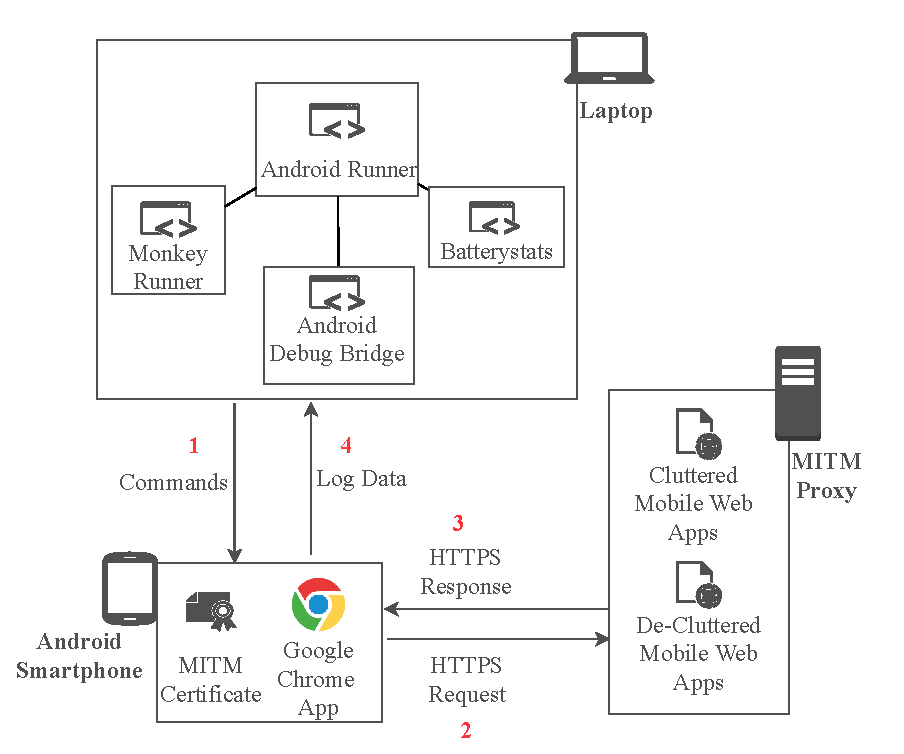
\includegraphics[width=9cm]{reportTemplate/figures/execution.pdf}
\caption{\textcolor{blue}{Experiment Execution}} \label{fig:deploymentview}
\end{figure}

The smartphone is connected to a laptop using Android Debug Bridge (adb)\footnote{\url{https://developer.android.com/studio/command-line/adb}}. The computer that we use to manage the experiment has an Intel i7 CPU (8th generation, 8 cores, and 4.2 GHz maximum clock speed) with 16 GB of RAM. Adb is a tool that allows communication between a development machine and an Android device. This communication entails information of the experiment configurations from the laptop to the smartphone and measurement data from the smartphone to the laptop. The Android smartphone and laptop are both connected to the same LAN. All the devices are in close proximity \textcolor{blue}{(less than a meter)} to the WiFi router (802.11ac standard and 5 GHz frequency band) to ensure minimum latency. The Android smartphone uses the Google Chrome web browser version \textcolor{blue}{{66.0.3359.158}} to access the internet and load the cluttered and de-cluttered mobile web apps. The researchers of the JSCleaner paper~\cite{chaqfeh2020jscleaner} cached the cluttered and de-cluttered mobile web apps, which they used for their research, on a proxy server and shared this proxy with us. In order to access the proxy server, the mitmproxy\footnote{\url{https://docs.mitmproxy.org/}} certificate \textcolor{blue}{is} installed on the smartphone. Mitmproxy is an HTTPS proxy that allows (among other features) interactive HTTPS requests. 

In order to \textcolor{blue}{execute} the experiment, we use Android Runner (AR)\footnote{\url{https://github.com/S2-group/android-runner}}. AR is a tool that facilitates the execution of measurement-based experiments on native apps and mobile web apps running on Android devices \cite{malavolta2020runner}. AR allows us to fill in the experiment configurations and setup after which it communicates this to the smartphone. After the experiment is conducted, AR stores the recorded measurement data on the laptop. AR utilizes Monkey Runner\footnote{\url{https://developer.android.com/studio/test/monkeyrunner}} to implement an API that grants control over the Android smartphone. We use Monkey Runner to construct a log of smartphone input commands. This log can be used to automate the interactions with the smartphone. \textcolor{blue}{Lastly, we use the Batterystats\footnote{\url{https://github.com/S2-group/android-runner/tree/master/AndroidRunner/Plugins/batterystats}} utility to measure the energy consumption. We chose this profiler as it was compatible with the used smartphone. Furthermore, Tan et al.~\cite{integrationtan} found an indication of Batterystats providing more accurate results of the power consumption compared to Trepn\footnote{\url{https://github.com/S2-group/android-runner/tree/master/AndroidRunner/Plugins/trepn}}. Batterystats is a plugin of AR.}

A high-level view of our experiment execution is visualized in Figure \ref{fig:deploymentview}. \textcolor{blue}{The experiment includes three main components: the \textit{Laptop}, \textit{Android Smartphone}, and \textit{MITM Proxy}. The experiment starts with sending commands from the \textit{Laptop} to the \textit{Android Smartphone} (step \textcolor{red}{1}). The connection between the \textit{Laptop} and the \textit{Android Smartphone} is established using \textit{Android Debug Bridge}. \textit{Monkey Runner} handles the automation of the external control of the smartphone (e.g. Terms and Conditions in browser app) and \textit{Batterystats} takes care of measuring the power consumption. These processes are orchestrated and managed by \textit{Android Runner}. Once the \textit{Android Smartphone} receives the commands, it requests (step \textcolor{red}{2}) the relevant \textit{Cluttered or De-Cluttered Mobile Web Apps} from the \textit{MITM Proxy}. The \textit{MITM Proxy} sends (step \textcolor{red}{3}), after checking the \textit{MITM Certificate}, the \textit{Cluttered or De-Cluttered Mobile Web Apps} to the \textit{Android Smartphone}. Lastly, the log data and measurement results are collected by \textit{Android Runner} (step \textcolor{red}{4}).}

After each run, the Google Chrome browser is cleared and closed. Then, the smartphone remains idle for \textcolor{blue}{2} minutes to ensure that all processes are finished. To guarantee the intrinsic variability of the experiment, each trial is repeated 15 times. We repeat this measurement for 10 randomly selected cluttered mobile web apps and their de-cluttered version.